\chapter{Virtualbox y adaptadores de red}

\section{Introducción}
\href{https://www.virtualbox.org/}{Virtualbox} es una herramienta de virtualización para crear máquinas virtuales de manera sencilla. Es multiplataforma por lo que se puede utilizar en Windows, MacOS y Linux y aparte, es \hyperlink{software_libre}{Software Libre}.

Este documento no va a entrar en detalle en cómo se crean las máquinas virtuales, sino que va a explicar los distintos modos y adaptadores de red que puede tener una máquina virtual en este sistema de virtualización.

\section{Adaptadores de red}
Virtualbox permite que cada máquina virtual cuente con hasta cuatro adaptadores de red, lo que comúnmente se llaman interfaces o NIC (network interface controller).

Al crear las máquinas virtuales sólo tienen un único adaptador activo y suele estar configurado en modo NAT, pero tal como se ve a continuación, en el desplegable se puede ver que existen otras opciones:

\begin{center}
    \vspace{-10pt}
    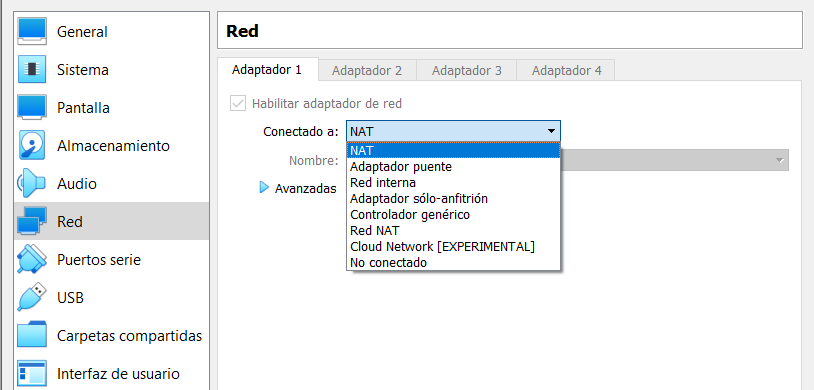
\includegraphics[frame,width=0.7\linewidth]{virtualbox_1.png}
    \vspace{-20pt}
\end{center}

En la \href{https://www.virtualbox.org/manual/ch06.html}{documentación oficial} aparece la explicación de los distintos modos, y es buena práctica leer y entender la documentación del software que utilizamos. También hay que entender que cada tipo de adaptador contará con una serie de ventajas y una serie de limitaciones que aparecen reflejadas en la documentación. Estos modos son comunes a otros  sistemas de virtualización (VmWare, Proxmox, …), pero el nombre o el modo de uso puede variar así como las posibles limitaciones que puedan existir.

A continuación se va a dar una pequeña introducción a cada tipo de adaptador.

\subsection{Adaptador puente}
Es el tipo de adaptador que se usará si queremos que las máquinas virtuales aparezcan en la red física como si fueran un equipo más. Para poder entenderlo de mejor manera, podríamos pensar que este tipo de adaptador lo que hace es crear un “switch virtual” entre las máquinas virtuales y el interfaz físico, por lo que es como si fueran un equipo más en la red física.

Si el equipo físico anfitrión cuenta con más de un NIC (por ejemplo, en un portátil el NIC por cable y el NIC wifi) tendremos que elegir en la máquina virtual sobre qué NIC queremos hacer el puente. En la siguiente imagen en el desplegable sólo se puede seleccionar un interfaz porque el equipo sólo cuenta con un NIC físico.

\begin{center}
    \vspace{-10pt}
    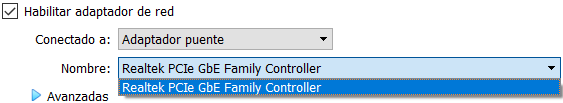
\includegraphics[frame,width=0.7\linewidth]{virtualbox_2.png}
    \vspace{-20pt}
\end{center}

Es el método utilizado cuando virtualizamos servidores, ya que podrán dar sus servicios a toda la red.

\begin{center}
    \vspace{-10pt}
    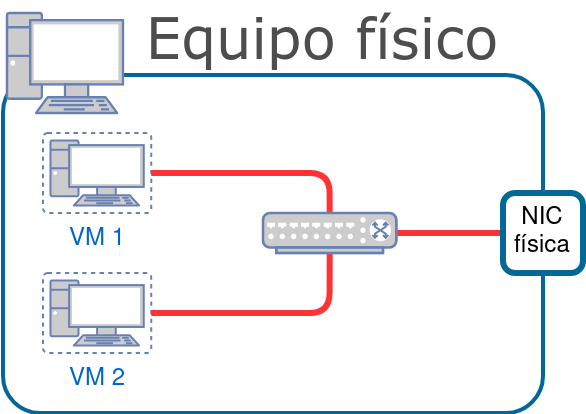
\includegraphics[width=7cm]{virtualbox-bridge.png}
    \vspace{-10pt}\captionof{figure}{Red como Adaptador Puente}
    \vspace{-20pt}
\end{center}

\subsection{NAT}
Cada máquina virtual contará con su propio “router virtual” que hará NAT, y por eso todas las máquinas virtuales que usen este modo suelen tener la misma IP, pero no pertenecen a la misma red.
Por defecto no se puede realizar conexión desde la red física al equipo virtualizado.

\begin{center}
    \vspace{-10pt}
    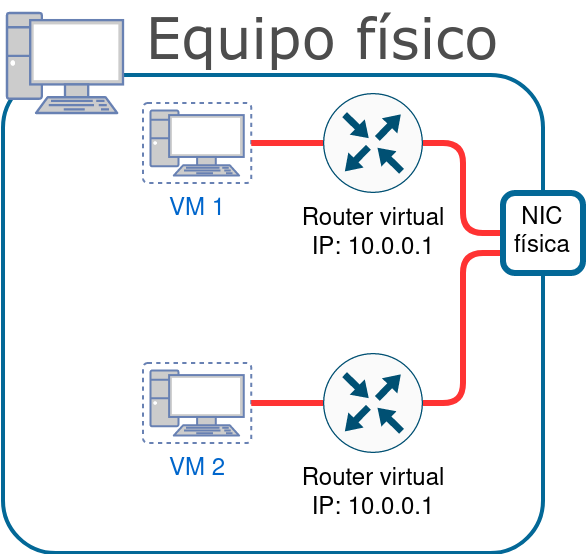
\includegraphics[width=7cm]{virtualbox-NAT.png}
    \vspace{-10pt}\captionof{figure}{Red en modo NAT}
    \vspace{-20pt}
\end{center}

\subsection{Red interna}
Este tipo de adaptador lo que hace es “crear” un “switch virtual” que unirá las distintas máquinas virtuales que estén conectadas al nombre de esa red interna.

En el siguiente ejemplo la VM1 tiene 2 NICs, cada una con una red interna distinta. La VM2 tiene un NIC conectado a una de las redes internas creadas previamente y VM3 está conectada a la otra red interna.

Virtualbox no se encarga de dar IPs en estas redes, por lo que deberemos configurar cada interfaz de la máquina virtual con el direccionamiento que nos interese.

Este método se utiliza si queremos comunicar máquinas virtuales entre sí y que estén aisladas, ya que no podrán conectarse con el exterior, ni siquiera con el propio equipo físico.

\begin{center}
    \vspace{-10pt}
    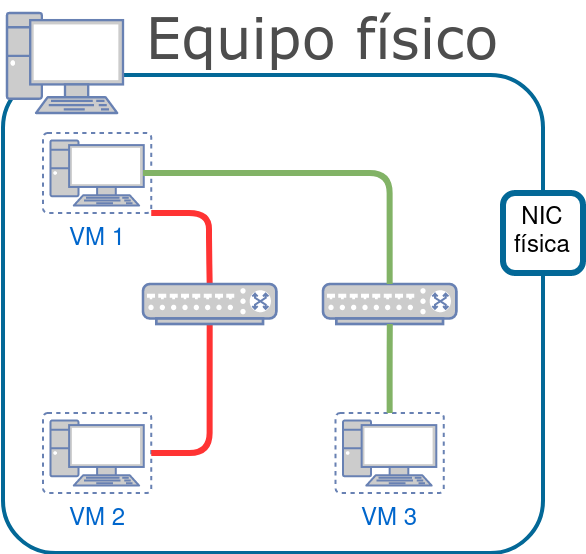
\includegraphics[width=7cm]{virtualbox-red_interna.png}
    \vspace{-10pt}\captionof{figure}{Red Interna}
    \vspace{-20pt}
\end{center}

\subsection{Red NAT}
Podría definirse como una mezcla de NAT y red interna. Las máquinas virtuales podrán pertenecer a una única red, se podrán comunicar entre ellas, estarán detrás de un NAT de la red física y se podrán comunicar con el exterior.

Para poder usar ese modo hay que crear la “red NAT” en Virtualbox yendo a “\textit{Archivo → Preferencias → Red}” y ahí se creará las redes NAT que queramos con el direccionamiento interno que nos interese.

\begin{center}
    \vspace{-10pt}
    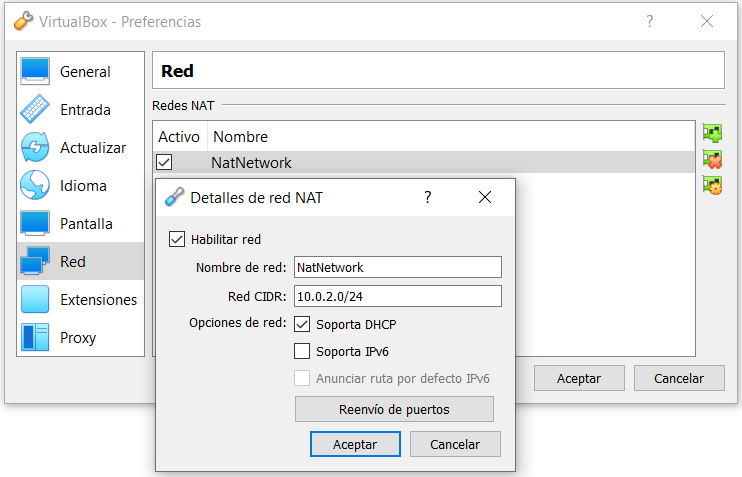
\includegraphics[width=8cm]{virtualbox-red-NAT_config.png}
    \vspace{-20pt}
\end{center}

A la hora de crear la máquina virtual y elegir la opción “Red NAT” se podrá elegir entre las redes creadas en el paso anterior.

\begin{center}
    \vspace{-10pt}
    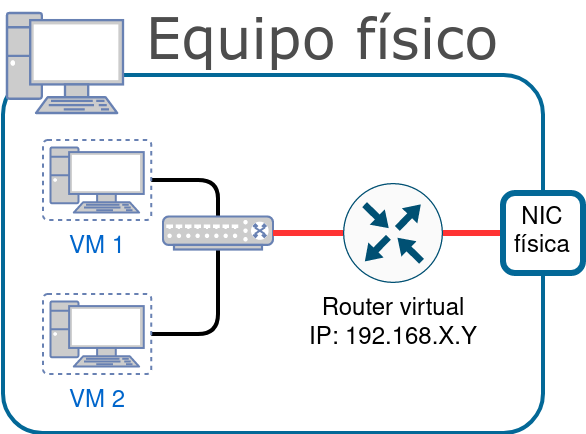
\includegraphics[width=7cm]{virtualbox-red-NAT.png}
    \vspace{-10pt}\captionof{figure}{Red NAT}
    \vspace{-20pt}
\end{center}

\subsection{Adaptador sólo-anfitrión}
Este tipo de adaptador es similar al de “red interna” pero con la posibilidad de comunicarse con el equipo físico anfitrión. En el equipo físico se crea un interfaz virtual y a través de él se podrá comunicar con las máquinas virtuales.

\begin{center}
    \vspace{-10pt}
    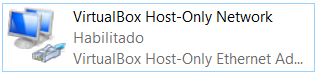
\includegraphics[width=7cm]{virtualbox-host_only_nic.png}
    \vspace{-20pt}
\end{center}

El direccionamiento que existe entre las VMs y el host se define en Virtualbox, dentro de “\textit{Archivo → \textbf{Administrador de red de anfitrión}}”. Las máquinas virtuales podrán coger IP de ese direccionamiento  por DHCP.

Mismo uso que “red interna” pero añadiendo la opción de comunicarnos con el host anfitrión.

\begin{center}
    \vspace{-10pt}
    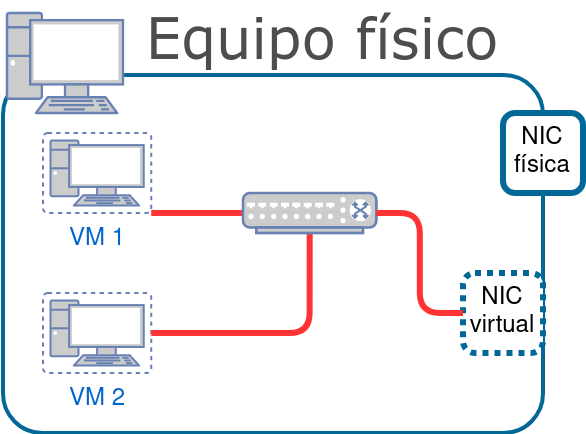
\includegraphics[width=7cm]{virtualbox-host_only.png}
    \vspace{-10pt}\captionof{figure}{Red en modo “Sólo Anfitrión”}
    \vspace{-20pt}
\end{center}

\section{Resumen de los adaptadores}
A continuación se expone una tabla que resume los distintos tipos de adaptadores que existen y la conectividad posible entre las máquinas virtuales que usan esos adaptadores y el host anfitrión (\href{https://www.virtualbox.org/manual/ch06.html#networkingmodes}{fuente}).

\begin{center}
    \vspace{-10pt}
    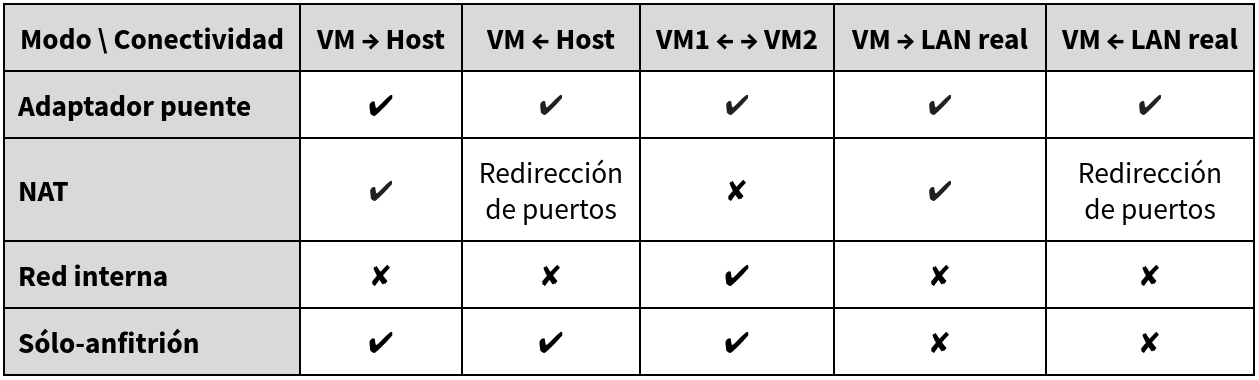
\includegraphics[width=\linewidth]{virtualbox_tabla.png}
    \vspace{-20pt}
\end{center}

En la \href{https://www.virtualbox.org/manual/ch06.html#natforward}{documentación} se explica cómo realizar la redirección de puertos.


\clearpage